\documentclass{article}
\usepackage{amsmath}
\usepackage{amssymb}
\usepackage{graphicx}
\pagestyle{empty}
\begin{document}
\raggedright\noindent
{\Large Linear independence}

\ \\

\begin{enumerate}
\item Find a vector $x_3$ so that $\{x_1, x_2, x_3\}$ are linearly independent.
\[
x_1 = \left( \begin{array}{c} 1 \\ 1 \\ 1\\ \end{array} \right) , \qquad x_2 = \left( \begin{array}{c} 3 \\ 0 \\ 2\\ \end{array} \right)
\]

\item More important than finding a specific solution, can you describe a general procedure for solving the problem above?

\item Can you find the matrix $M\in {\Bbb R}^2$ that stretches the plane away from the origin along the the line $y=x$?\\ \ \\
{
    \centering
    \begin{minipage}{2.1in}
      \centering
      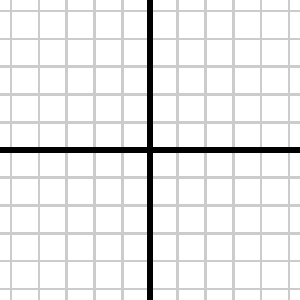
\includegraphics[width=1.5in]{xyplane.pdf}
      %\caption{Domain}
    \end{minipage}
    $\to$
    \begin{minipage}{2.1in}
      \centering
      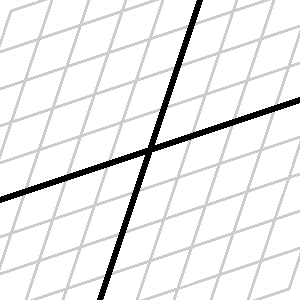
\includegraphics[width=1.5in]{xyplane-stretch.pdf}
      %\caption{Range}
    \end{minipage}
}\\ \ \\ \ \\
Hint: Which vectors will be transformed by a scalar?  That is, for which $x$ is
\[ Mx = [\text{stretch factor}]x\]
\end{enumerate}

{\large Submission instructions}
\begin{enumerate}
\item Create a folder in your repo called {\tt linear-independence}
\item Within the folder, create a pdf or html file called {\tt solution}
\end{enumerate}

\end{document}